\begin{figure}
\centering
\begin{subfigure}[b]{\linewidth}
    \hfill
    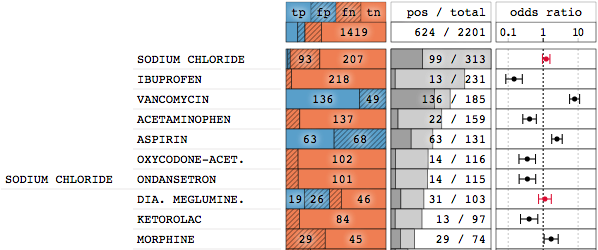
\includegraphics[height=7em]{explainer/expl_10_size}
    \caption{~Ordered by ``total" size showing the most common explanations.}
    \label{figs:expl_10_size}
\end{subfigure}
\\
\begin{subfigure}[b]{\linewidth}
    \hfill
    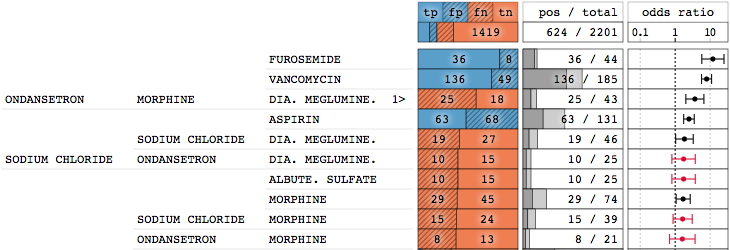
\includegraphics[height=7em]{explainer/expl_10_or_pos}
    \caption{~Ordered by ``odds ratio" showing significantly positive explanations.}
    \label{figs:expl_10_or_pos}
\end{subfigure}%
\\
\begin{subfigure}[b]{\linewidth}
    \hfill
    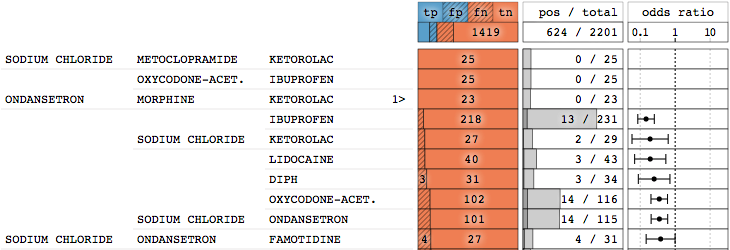
\includegraphics[height=7em]{explainer/expl_10_or_neg}
    \caption{~Ordered by reverse ``odds ratio" showing significantly negative explanations.}
    \label{figs:expl_10_or_neg}
\end{subfigure}%
\\
\begin{subfigure}[b]{\linewidth}
    \hfill
    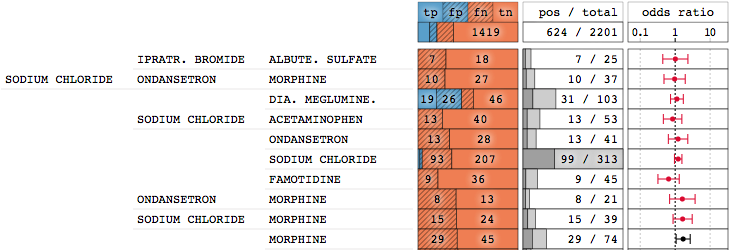
\includegraphics[height=7em]{explainer/expl_new_uncertain}
    \caption{~Ordered by ``uncertainty" showing item subsets whose predictions are not significant.}
    \label{figs:expl_10_uncertain}
\end{subfigure}
\caption{
Showing different orders in the \textbf{\tabB} for addressing the goals (G2 \& G3) in the case study (Section~\ref{sec:case_study}). The initial dataset is filtered for explanations with $> 20$ data items.
% The \textbf{\tabB} showing the initial case study dataset (see Section~\ref{sec:case_study}) filtered for explanations with $> 20$ data items.
}
\end{figure}